\chapter{基于Kagome晶格的声学哈密顿量推导及边界条件对拓扑态的影响研究}

\section{引言}

\section{Kagome晶格与声学结构类比}

\begin{figure}[h!]
  \centering
  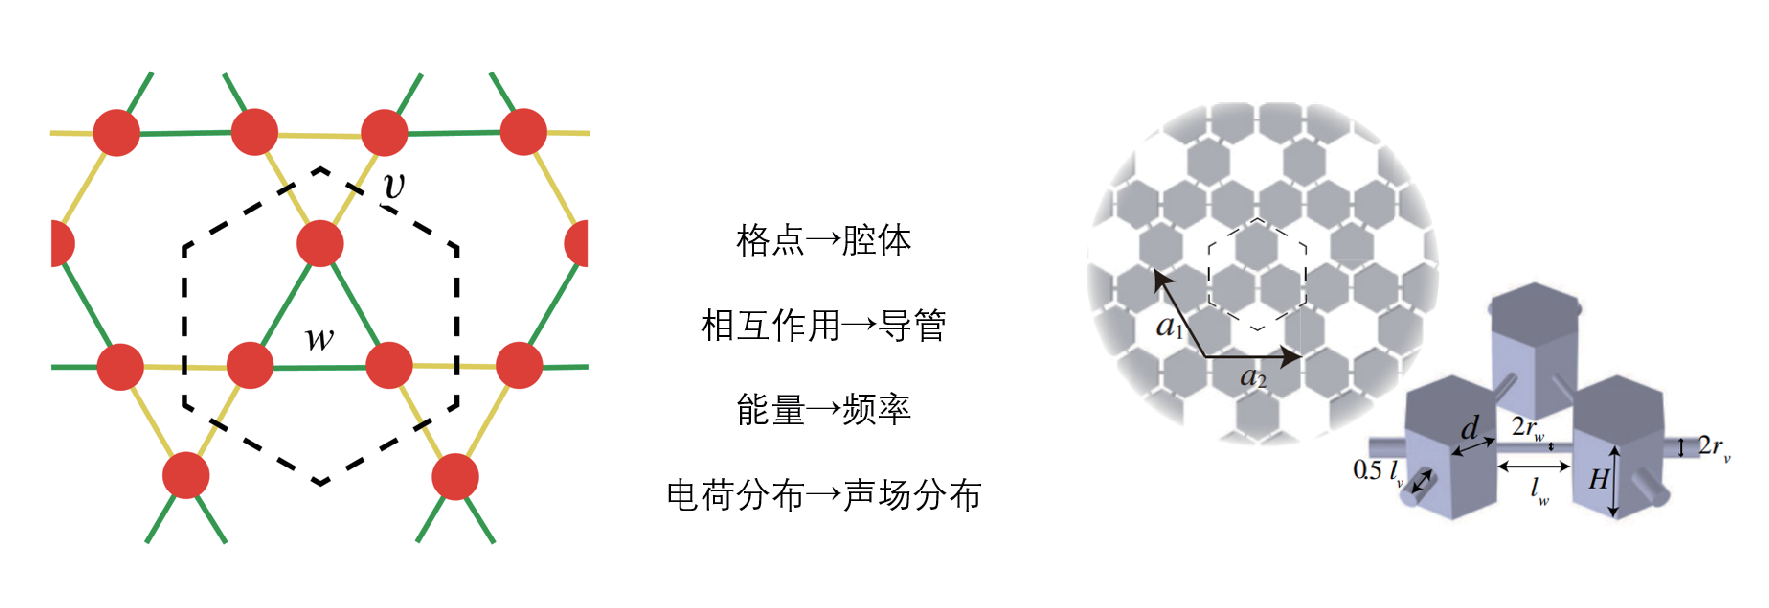
\includegraphics[width=1\textwidth]{images/fig3-1.eps} 
  \caption{以Kagome结构为例,电子系统与声学系统存在显著的相似性。}
  \label{fig_3_1}
\end{figure}

在物理学中,电子系统与声学系统存在显著的相似性。电子系统里,格点、相互作用、能量、电荷分布是关键要素;而在声学系统中,可类比为腔体、导管、频率、声场分布。以图\ref{fig_3_1}的Kagome晶格为例,以下是电子系统和声学系统中几个要素的相似性详细解释:
\begin{itemize}
  \item 格点与腔体:在电子系统的晶格模型中,格点是电子所处的位置,电子在这些格点上具有一定的能量状态和量子特性。格点的排列和相互关系决定了电子的能带结构等重要物理性质。而在声学系统中,我们可以把单个腔体看作是一个共振单元,它也具有共振频率和对应的共振模式。而使用周期排列的声学腔体,可以模仿电子晶格空间排列,构造相同的空间对称性。二者在离散化的单个单元共振和多个单元的空间排列上,存在一定的相似性。
  \item 电子系统的相互作用与声学导管:在电子系统的晶格模型中,电子在晶格中的跳跃等过程可以看作是一种相互作用,它决定了电子在不同格点之间的转移和能量传递。在声学系统中,我们可以在腔体之间连接导管,为不同腔体提供相互作用,并通过调节导管的参数实现对这种相互作用的大小和正负符号的调节。二者在单元和单元的相互作用上存在一定的相似性。
  \item 能量与频率:在电子系统中,薛定谔方程用于求解电子能量的本征值问题,其能量以离散本征值呈现,相应本征向量描述电子运动状态 。当处于周期结构时,电子会形成能带,其特性受晶格周期性影响。在声学系统里,波动方程的求解同样属于本征值问题,频率(或者频率的平方)作为本征向量,其离散取值决定声波传播模式。在周期结构的声学体系中,声波也会形成类似的能带结构,该结构与声学单元的周期性排列密切相关。二者在本征值问题架构及周期结构下形成能带的特性上,展现出显著的相似性。 
  \item 电荷分布与声场分布:在电子系统中,电荷分布反映了电子于空间的分布态势,它与电子的能量状态、相互作用及外部电场紧密相连,电荷分布的不均匀会引发电场等物理效应,对电子系统的电学性质和物理行为产生影响。在声学系统里,声场分布体现了声波在空间中的强度、相位分布状况,腔体和导管的结构以及声波传播特性致使声场在空间呈现不同分布模式。二者相似之处在于,它们均是描述各自系统内物理量在空间的分布,且这种分布都会显著影响系统与其他物质的相互作用,以及整个系统的性能表现。特别地,在拓扑绝缘体的研究中,我们可以观测二者的场分布,从而观测其拓扑性质。 
\end{itemize}

从类比的相似性出发,我们构造了如图\ref{fig_3_1}所示的声学结构。图中周期结构以C$_{3}$对称性排列,其中$a_1$和$a_2$是两个方向晶格基矢的大小,用于描述晶格的周期性结构。右侧展示了单个元胞内的三维结构,包含六边形腔体,其边长为$d$,高度为$H$。$l_w$和$l_v$分别对应胞内耦合的导管和胞间导管的长度,$r_w$和$r_v$是分别对应胞内耦合的导管和胞间导管的半径。从直觉上而言,当连接两个腔体的导管的长度更短,横截面积更大,此时两个腔体之间的相互作用更大,对应电子系统中更大的格点间的跳跃。

\section{Kagome晶格的声学哈密顿量}

\begin{figure}[h!]
  \centering
  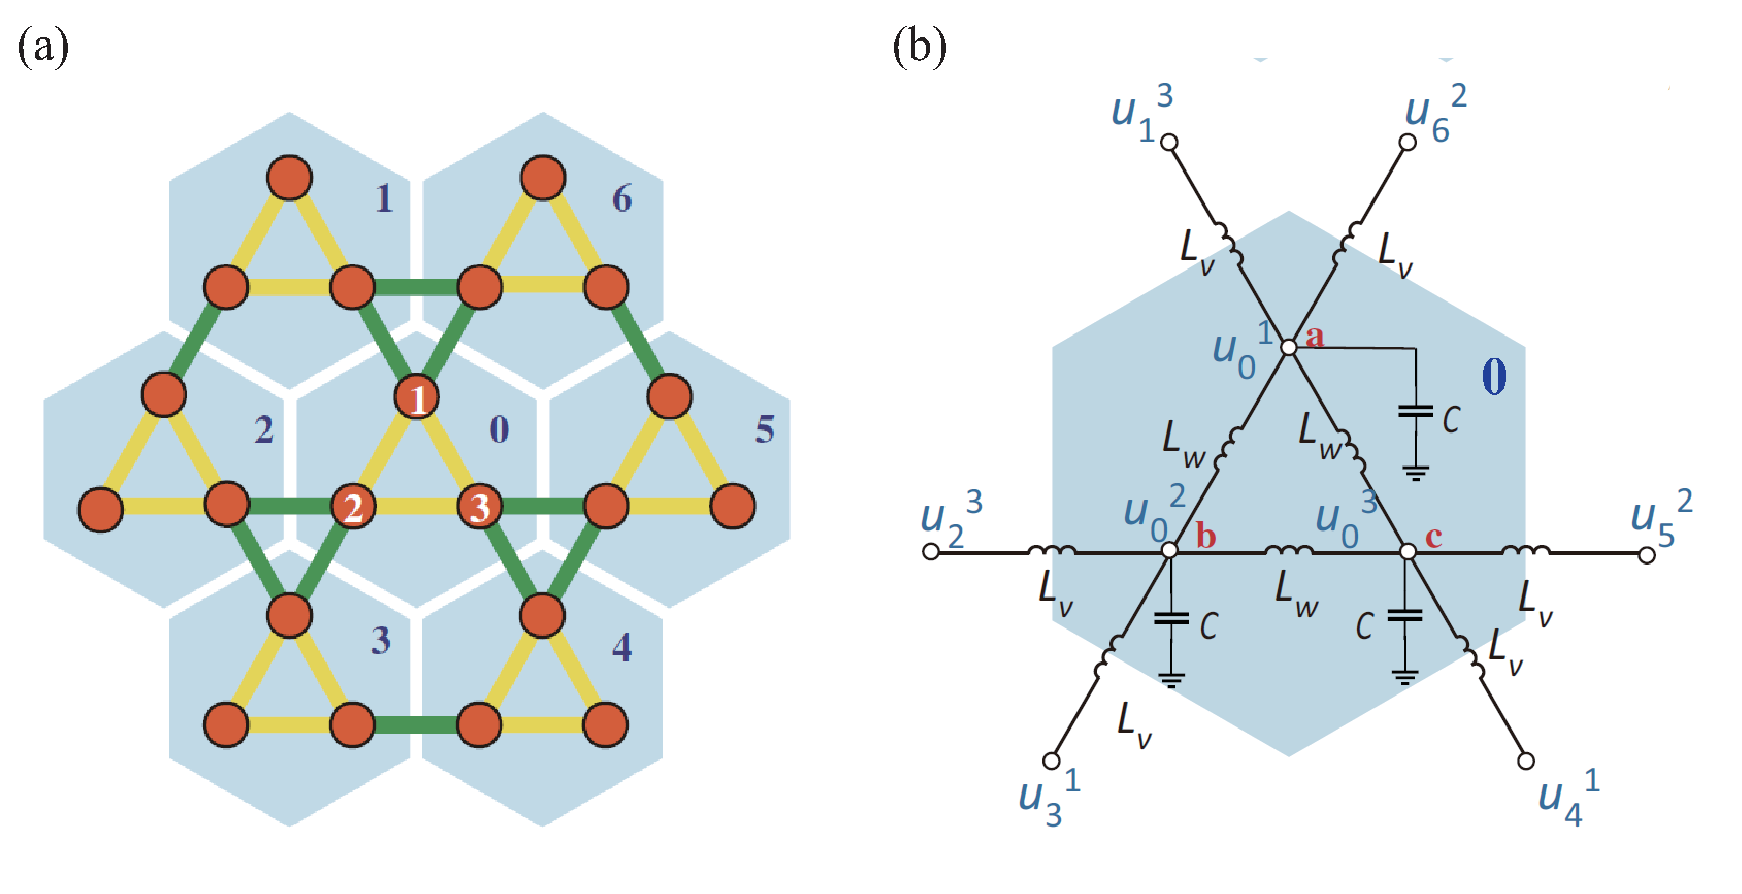
\includegraphics[width=1\textwidth]{images/fig3-2.eps} 
  \caption{Kagome声学系统的等效电路:
  (a)元胞Kagome晶格结构,其中晶格0居中,周围相邻的晶格分别编号为1到6。(b)晶格0的等效电路图。
  }
  \label{fig_3_2}
\end{figure}

如上一节所述,电子系统和声学系统有着相似性,我们可以构造声学腔管结构来类别电子Kagome晶格,也可以通过直觉调控其胞间和胞内的相互作用。在本节中,从声电类比方法出发,我们在亚波长尺度下从传统声学的角度严格推导出具有二维Kagome晶格的声共振系统的哈密顿量,从而揭示理论模型中的胞内或胞间跳跃与实际物理系统中的声学参数之间的联系。

首先,我们可以通过声学-电学类比来定义声学系统的 lumped 参数模型,单个单元的等效电路图如图\ref{fig_3_2}所示。在该电路模型中,腔体被表示为电容 \( C \),波导被表示为电感 \( L_v \) 和 \( L_w \)。具体公式如下:
\[
C = \frac{V}{\rho c^2}
\]
\[
L_v = \frac{\rho (l_v + 1.7r_v)}{\pi r_v^2}, \quad L_w = \frac{\rho (l_w + 1.7r_w)}{\pi r_w^2}
\]
其中,\( V \) 是腔体的体积,\( \rho \) 是空气的密度,\( c \) 是声速,\( r_v \) 和 \( r_w \) 分别是波导的半径,\( l_v \) 和 \( l_w \) 是它们的长度。


通过应用基尔霍夫电流定律,我们可以得到了描述声学波动的方程。对于周期性结构,腔体的声压在每个晶格点处满足如下方程:
\[
- (2w + 2v) u_1^0 + w u_2^0 + w u_3^0 + v u_2^6 + v u_3^1 = \omega^2 u_1^0
\]
\[
- (2w + 2v) u_2^0 + w u_3^0 + w u_1^0 + v u_3^2 + v u_1^3 = \omega^2 u_2^0
\]
\[
- (2w + 2v) u_3^0 + w u_1^0 + w u_2^0 + v u_1^4 + v u_2^5 = \omega^2 u_3^0
\]
其中,\( u_n^m \) 表示第 \( n \) 个腔体在第 \( m \) 个晶格上的声压,\( w = -\frac{1}{L_v C} \),\( v = -\frac{1}{L_w C} \) 是与腔体和波导的物理参数相关的系数,\( \omega \) 是角频率。


通过上述方程,可以将哈密顿量表示为矩阵形式。在周期性结构下,哈密顿量 \( H_0(k) \) 以矩阵的形式表示为:
\[
H_0(k) =
\begin{pmatrix}
-2w - 2v & w + v e^{i k \cdot (a_1 + a_2)} & w + v e^{i k \cdot a_1} \\
w + v e^{-i k \cdot (a_1 + a_2)} & -2w - 2v & w + v e^{-i k \cdot a_2} \\
w + v e^{-i k \cdot a_1} & w + v e^{i k \cdot a_2} & -2w - 2v
\end{pmatrix}
\]
这里,\( k \) 是布里渊区内的波矢,\( a_1 \) 和 \( a_2 \) 是晶格常数。


考虑到实际声学系统的边界条件,文章进一步推导了边界对哈密顿量的影响。对于有限结构,硬边界和软边界条件分别影响哈密顿量的对角项。

- **硬边界条件**:对于硬边界,腔体的对角项变为:
  \[
  - (2w + v)
  \]
  
- **软边界条件**:对于软边界,腔体的对角项变为:
  \[
  - (2w + 2v)
  \]


文章进一步通过计算系统的拓扑极化,来揭示哈密顿量与拓扑相之间的关系。极化 \( p \) 的计算通过下式给出:
\[
e^{-i \pi p} = \prod_{n \in \text{occ}} \theta_n(K) \theta_n(\Gamma)
\]
其中,\( \theta_n(k) = \langle u_n(k) | R_3 | u_n(k) \rangle \) 是通过三重对称操作 \( R_3 \) 计算得到的本征值,\( n \) 是占据的能带,\( K \) 和 \( \Gamma \) 是高对称点。


通过上述推导,文章揭示了软边界条件如何保留系统的拓扑特性,特别是角落态的存在,这些角落态与电子系统中的零能态相对应。

总结而言,哈密顿量的推导通过声学电学类比、基尔霍夫电流定律以及周期性结构的布洛赫波函数方法,详细描述了声学拓扑晶体绝缘体的物理特性,同时揭示了边界条件对拓扑态的关键作用。


\section{Kagome晶格体能带与拓扑相变}

\section{Kagome晶格的边界态和角态}

\section{边界条件对拓扑态的影响}